%%%%%%%%%%%%%%%%%%%%%%%%%%%%%%%%%%%%%%%%%
%%% HYPERRIDE Reporting Template
%%%%%%%%%%%%%%%%%%%%%%%%%%%%%%%%%%%%%%%%%
\documentclass[12pt,a4paper,ngerman]{report}
%\documentclass[11pt]{report}

\usepackage{hyperride}		% HYPERRIDE specific definitions and styles  
\usepackage{hyperref}
\usepackage[utf8]{inputenc}	% UTF8 package
\usepackage[T1]{fontenc}
\usepackage{tgbonum}
\usepackage{textcomp}		% common special chars
\usepackage{amsmath}		% math formula
\usepackage{fancybox}
\usepackage{anyfontsize}	% fonts
\usepackage{lipsum}
\usepackage{float}
\usepackage[normalem]{ulem}
\usepackage{cleveref}
\usepackage{siunitx}
\usepackage[printonlyused]{acronym}
\usepackage{pdfpages}


\hypersetup{
	pdftitle={Bahnumrichter},
	pdfauthor={[Names of co-authors (partners short names)]},
	pdfkeywords={Periodic Report, European Union (EU), H2020, Project, HYPERRIDE, GA 957788},
}

\graphicspath{ {graphics/} }


%%%%%%%%%%%%%%%%%%%%%%%%%%%%%%%%%%%%%%%%%
%%% Definitions
%%%%%%%%%%%%%%%%%%%%%%%%%%%%%%%%%%%%%%%%%

%\def\todo#1{{\color{hyperridered}\textbf{TODO:} ``#1''}}
\def\hyperride{HYPERRIDE}

% CHANGE %'s below to make subsection headings visible/invisible in TOC
%\newcommand{\xsubsubsection}[1]{\subsection{#1}}
%\newcommand{\xsubsubsection}[1]{\subsubsection{#1}}

\begin{document}

%%%%%%%%%%%%%%%%%%%%%%%%%%%%%%%%%%%%%%%%%

%%% URL style same as regular text
%%%%%%%%%%%%%%%%%%%%%%%%%%%%%%%%%%%%%%%%%
	
\urlstyle{same}

%%%%%%%%%%%%%%%%%%%%%%%%%%%%%%%%%%%%%%%%%
%%% Deliverable Information
%%%%%%%%%%%%%%%%%%%%%%%%%%%%%%%%%%%%%%%%%

% Project Meta Information
\ProjectFullTitle{}
\ProjectAcronym{Test}
\ProjectRefNo{957788}


% Report Number, use either "1", "2", or "3" for the corresponding reporting period
\delivNumber{0}

% Period covered by the report
\delivFrom{dd/mm/yyyy}
\delivTo{dd/mm/yyyy}

% Report Responsible Partner
\delivResponsible{AIT Austrian Institute of Technology (AIT)} 

% Report Version, Contractual and Actual Date, Dissemination Level, Type
\delivVersion{vn.n}
\ContractualDate{dd/mm/yyyy}
\ActualDate{dd/mm/yyyy}

% List of Main Authors (usually from the responsible partner)
\delivAuthor{[Names of co-authors (partners short names)]}

% List of Co-Authors (all other co-authors should be listed here)
\delivFPAuthor{[Names of co-authors (partners short names)]}

% Report Status
\delivStatus{d} %% d = draft, f = final, s = submitted

%%%%%%%%%%%%%%%%%%%%%%%%%%%%%%%%%%%%%%%%%
%%% Change Log
%%%%%%%%%%%%%%%%%%%%%%%%%%%%%%%%%%%%%%%%%

\istChange{dd/mm/yyyy}{v1.0}{Name (Partner short name)}{Draft report template}
\istChange{}{}{}{}

%%%%%%%%%%%%%%%%%%%%%%%%%%%%%%%%%%%%%%%%%
%%% Cover Page
%%%%%%%%%%%%%%%%%%%%%%%%%%%%%%%%%%%%%%%%%

\makecover

%%%%%%%%%%%%%%%%%%%%%%%%%%%%%%%%%%%%%%%%%
%%% Table of Contents
%%%%%%%%%%%%%%%%%%%%%%%%%%%%%%%%%%%%%%%%%

\clearpage
\fancypagestyle{plain}{}
\settableofcontents
\tableofcontents

%%%%%%%%%%%%%%%%%%%%%%%%%%%%%%%%%%%%%%%%%
%%% List of Figures
%%%%%%%%%%%%%%%%%%%%%%%%%%%%%%%%%%%%%%%%%

\clearpage
\setlistoffigures
\listoffigures

%%%%%%%%%%%%%%%%%%%%%%%%%%%%%%%%%%%%%%%%%
%%% List of Tables
%%%%%%%%%%%%%%%%%%%%%%%%%%%%%%%%%%%%%%%%%

\clearpage
%\setlistoftables
%\listoftables

%%%%%%%%%%%%%%%%%%%%%%%%%%%%%%%%%%%%%%%%%
%%% List of Abbreviations
%%%%%%%%%%%%%%%%%%%%%%%%%%%%%%%%%%%%%%%%%

%%%%%%%%%%%%%%%%%%%%%%%%%%%%%%%%%%%%%%%%%
%%% List of Abbreviations
%%%%%%%%%%%%%%%%%%%%%%%%%%%%%%%%%%%%%%%%%

\clearpage
\section*{List of Abbreviations}
\label{sec:abbreviations}

\begin{acronym}[ABCDEF]
	\acro{4QS}{Vierquadrantensteller}
\end{acronym}

%%%%%%%%%%%%%%%%%%%%%%%%%%%%%%%%%%%%%%%%%

%%%%%%%%%%%%%%%%%%%%%%%%%%%%%%%%%%%%%%%%%
%%% Deliverable Content
%%%%%%%%%%%%%%%%%%%%%%%%%%%%%%%%%%%%%%%%%

% Allgemeine Einleitung und Erklärung
\clearpage
\section{Allgemeine Projekt Beschreibung}
In der folgenden Konzeptionierung wird eine Umrichteranlage an $\SI{110}{\kV}$, im $\SI{50}{\Hz}$ Drehstrom Netz für das $\SI{110}{\kV}$,$\SI{16.7}{\Hz}$ Bahnnetz ausgelegt.
Die Einspeisung aus dem Drehstromnetz erfolgt über einen Netztrafo 


% Begründen Sie den Einsatz von Statischen Umrichtern zur Bahnstromversorgung im
% Vergleich zu alternativen Konzepten.
% Berücksichtigen Sie Vor- und Nachteile sowohl aus technischer und kommerzieller Sicht.
% Umfang eine einer Seite A4

\clearpage
\section{Konzeptionsvergleich zu Bahnumrichteranlage}
\label{sec:konzept_vergleich}

%%%%%%%%%%%%%%%%%%%%%%%%%%%%%%%%%%%%%%%%%
%%% Section content, please change!
%%%%%%%%%%%%%%%%%%%%%%%%%%%%%%%%%%%%%%%%%
Im Folgendem werden insbesondere 



\todo{Include in this section whether the information on section 2.1 of the DoA  (how your project will contribute to the expected impacts) is still relevant or needs to be updated. Include further details in the latter case.}

%%%%%%%%%%%%%%%%%%%%%%%%%%%%%%%%%%%%%%%%%


%%%%%%%%%%%%%%%%%%%%%%%%%%%%%%%%%%%%%%%%%
%%% References
%%%%%%%%%%%%%%%%%%%%%%%%%%%%%%%%%%%%%%%%%

\clearpage
%\bibliography{literature/references}
%\bibliographystyle{apacite}

%%%%%%%%%%%%%%%%%%%%%%%%%%%%%%%%%%%%%%%%%
%%% Appendix
%%%%%%%%%%%%%%%%%%%%%%%%%%%%%%%%%%%%%%%%%

\appendix

%%%%%%%%%%%%%%%%%%%%%%%%%%%%%%%%%%%%%%%%%
%%% Appendix A. Document Guidelines
%%%%%%%%%%%%%%%%%%%%%%%%%%%%%%%%%%%%%%%%%

\clearpage
\section*{Appendix A. Document Guidelines}
\addcontentsline{toc}{section}{Appendix A. Document Guidelines}
\label{sec:appendix-a}

%%%%%%%%%%%%%%%%%%%%%%%%%%%%%%%%%%%%%%%%%
%%% Section content, please change!
%%%%%%%%%%%%%%%%%%%%%%%%%%%%%%%%%%%%%%%%%

\subsection*{A.1. Report Titles}
\label{sec:appendix-a1-report-titles}
\addcontentsline{toc}{subsection}{A.1. Report Titles}

Deliverables have a title that is defined in the \ac{DoA}. This title is referred to as the full title of the deliverable. Please stick to the official spelling. It has turned out useful to also have a short title (max 60 characters) for each deliverable, as it can be cumbersome if one always has to use the full title. 

\subsection*{A.2. File Naming}
\label{sec:appendix-a2-file-naming}
\addcontentsline{toc}{subsection}{A.2. File Naming}

The project will generate many documents (deliverable reports) and versions of these reports. It is beneficial to consistently use an agreed file naming format. 

\textit{HYPERRIDE-Dnn-ShortTitle-Status-vn.n.Extension}

\begin{itemize}
	\item Notice the hyphen between the various elements of the file name.
	\item {\bf \hyperride{}}: Each \hyperride{} report should be preceded by the project acronym. Notice, there is only one correct spelling of the acronym: ‘\hyperride{}’. 
	\item {\bf Dn.n}: Indicates the deliverable identifier, e.g., ‘D34’ for ‘D3.4’ following the numbering of the \ac{DoA} (Part A of Annex 1 of the Grant Agreement). Notice, there is no dot between the two parts of the deliverable number.
	\item {\bf ShortTitle}: This should be based on the formal short title of deliverables but ‘contracted’ into a single (no spaces) character string using Java class naming convention, e.g., ‘ExploitationPlan’,  or ‘ProjectWebSite’. Avoid underscore, space and other unusual characters.
	\item {\bf Status}: 
	\begin{itemize}
		\item \textit{draft} = Draft Version – indicates that the drafting of the report is in progress; 
		\item \textit{final} = Final Version as checked and updated by the reviewers/WP leader/quality manager; 
		\item \textit{submitted} = submitted version as submitted to the EC by the project coordinator/administrator.
	\end{itemize}
	\item {\bf vn.n}: The version of the report starting from v1.0. 
	\item {\bf Extension}: File extension, e.g., ‘docx’ for Microsoft Word and ‘pdf’ for Portable Document Format. 
\end{itemize}

Examples:

\begin{itemize}
	\item HYPERRIDE-D82-InternalCommunication-draft-v1.0.docx
	\item HYPERRIDE-D84-QualityAssurancePlan-submitted.pdf
\end{itemize}

\subsection*{A.3. Change Log}
\label{sec:appendix-a3-change-log}
\addcontentsline{toc}{subsection}{A.3. Change Log}

The Change Log is there to keep track of the changes made to the document. Whenever changes are made to the document, a new version should be created and the changes should be briefly summarised in the Change Log. We anticipate a minimum of three phases of Change Log entries. (1) The researcher responsible for the given Deliverable enters the changes as he/she develops the document. (2) The two reviewers register the changes made in the quality assurance phase. Once the responsible researcher passes the report on to the Project Coordinator, the status should be changed from ‘draft’ to ‘final’. (3) The Project Coordinator submits the report to the EC, the status should be changed from ‘final’ to ‘submitted’.

\subsection*{A.4. Document Formatting}
\label{sec:appendix-a4-document-formatting}
\addcontentsline{toc}{subsection}{A.4. Document Formatting}

\subsubsection*{A.4.1. Headings}
\label{sec:appendix-a41-headings}

Like in many journals and books, it is a good practice not to use more than 3 levels of headings. If you really need more, then by all means do so, but you may first consider how to structure the document with a maximum of three heading levels. 

Use the following capitalisation style for all headings: All terms should be capitalised and do not use a full stop at the end.

\subsubsection*{A.4.2. Captions and Citations}
\label{sec:appendix-a42-captions-and-citations}

Use the following for captions and cross referencing:

\begin{itemize}
	\item ‘Table 1’ for tables, not ‘table 1’ or ‘Tab. 1’, etc.
	\item ‘Figure 1’ for figures, not ‘figure 1’ or ‘Fig. 1’, etc.
	\item ‘Section 1.1.1’ to cross-reference other sections, not ‘section 1.1.1’ or ‘S. 1.1.1’, etc.
\end{itemize}

Do not abbreviate the word ‘Equation’ to ‘eq’, ‘Eqn’, etc.

Table captions should be placed above the table and figure captions should be placed below the figure. The captions should succinctly describe the content of the table or figure.

\subsubsection*{A.4.3. Tables}
\label{sec:appendix-a43-tables}

Producing informative tables is not easy. Avoid grid lines around each table cells (typical for people with little experience in drafting technical papers). The table below (\Cref{tab:graphicastable}) is a good example how tables should look like. Make sure that caption appears on the same page as the table. The table caption is above the table!

The table caption should follow the sentence style layout and end with a full stop. The caption as well as the table should be centred.

Each table must be introduced in the deliverable text. Make sure that cross references to tables are correct before submitting the deliverable.

\begin{table}[htb]
	\centering
	\caption{Summary of properties of different modelling formalisms. The table below is inserted as graphic.}
	\label{tab:graphicastable}
	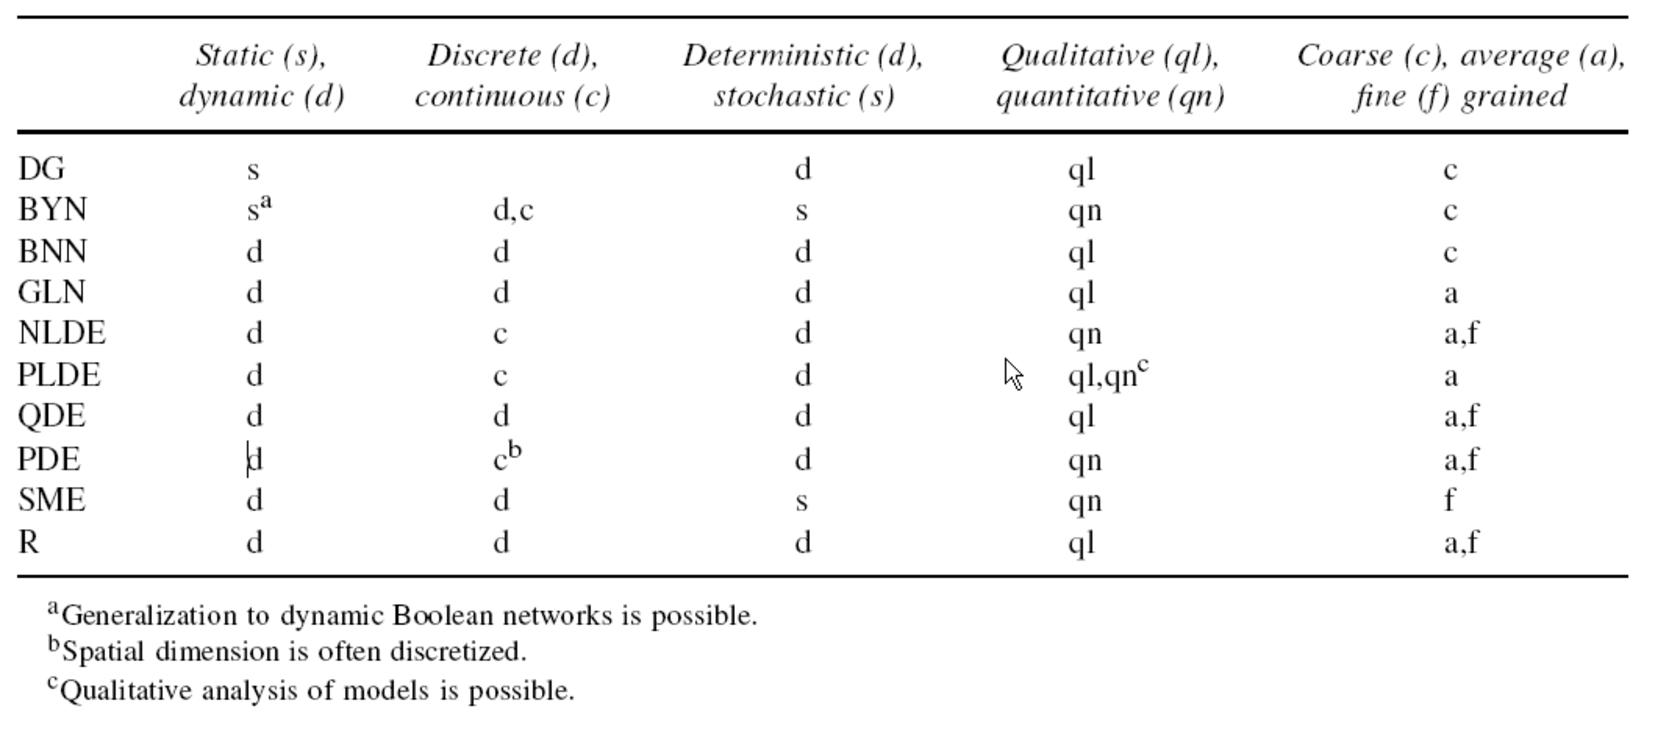
\includegraphics[width=1.00\linewidth]{graphics/graphicastable}  
\end{table}

The same (simplified) table using the \LaTeX\ table feature is shown below (\Cref{tab:latextable}).

\begin{table}[htb]
	\centering
	\caption{Summary of properties of different modelling formalisms. The table below is produced using \LaTeX's {\tt table} environment.}
	\label{tab:latextable}
	\begin{tabular}{cccccc}
		\hline
		& Static & Discrete & Deterministic & Qualitative & Coarse \\
		\hline
		DG & s &  & d & ql & c \\
		BYN & s & d,c & s & qn & c\\
		BNN & d & d & d & ql & c\\
		GLN & d & c & d & qn & a,f\\
		\hline
	\end{tabular}
\end{table}

\subsubsection*{A.4.4. Figures}
\label{sec:appendix-a44-figures}

Good figures/diagrams are even more difficult to produce than tables. Figures should contain legends explaining the symbols in the figure. Avoid surrounding the figure with a box outline. If there are different parts of a figure (e.g., (a), (b), (c)), indicate these clearly. Make sure that the labels within a figure/diagram are spelled consistently within the figure/diagram and are also consistently spelled in the text. Make sure that caption appears on the same page as the figure. The figure caption is below the figure. See an example of a figure and its caption below (\Cref{fig:figure}).

Each figure must be introduced in the deliverable text. Make sure that cross references to figures are correct before submitting the deliverable.

The figure caption should follow the sentence style layout and end with a full stop. The figure caption as well as the figure should be centred.

\begin{figure}[htb]
	\centering
	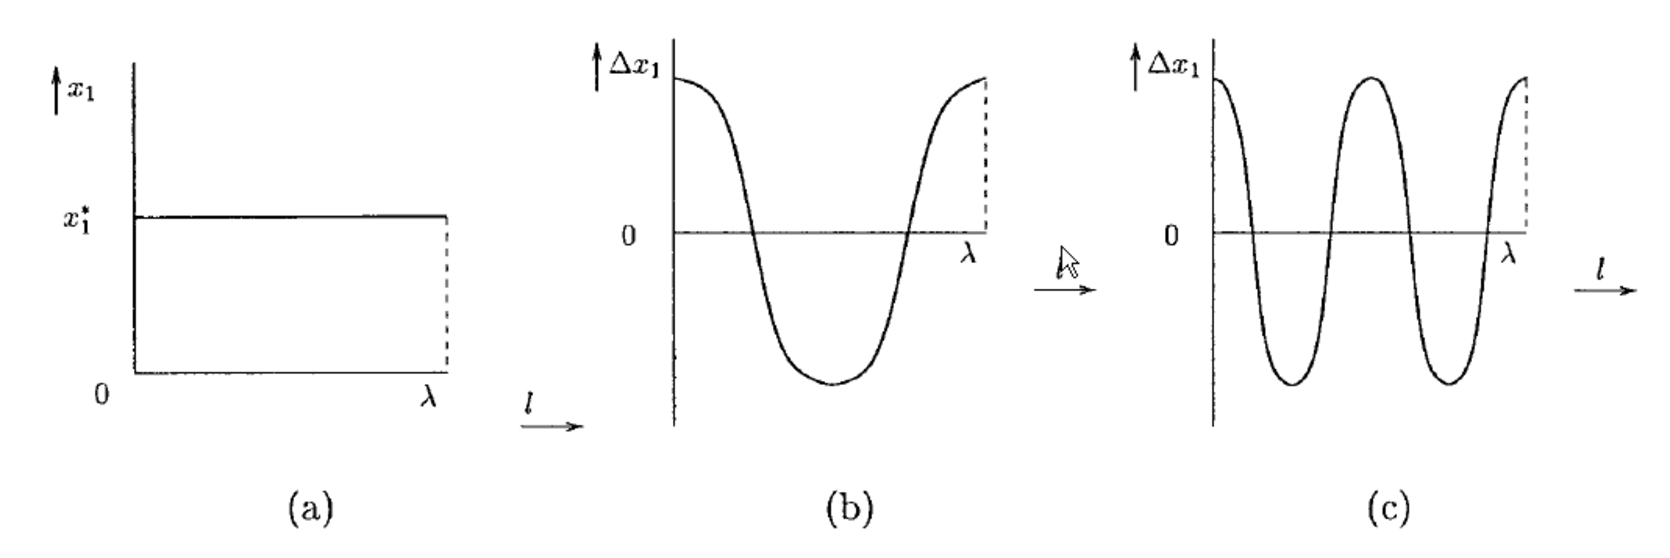
\includegraphics[width=.89\linewidth]{graphics/figure}
	\caption{Caption caption caption caption caption caption caption caption caption. (a) Caption caption caption, (b) Caption caption caption, (c) Caption caption caption.}
	\label{fig:figure}
\end{figure}

\subsubsection*{A.4.5. Footnotes}
\label{sec:appendix-a45-footnotes}

This\footnote{The footnote is at the bottom of the same page where the footnote is cited and the font size is only 9 pt. Footnotes are useful to for including nasty-looking long Web references which would look terrible if used in the main flow of the text.} is a footnote.

\subsection*{A.5. Language and Notation}
\label{sec:appendix-a5-language-notation}
\addcontentsline{toc}{subsection}{A.5. Language and Notation}

There are a few things we should consider when writing documents in terms of language. The question is not deeply philosophical in the sense of whether one or the other approach is fundamentally correct (or wrong). It is more the case of maintaining a certain level of consistency across the project.

Since British/UK English is the official version of English within the EC, we should by default use UK English spelling (and adopt a spell-checker set to UK English). Nevertheless, US spelling is also fine – the main issue to ensure is to be consistent within a given deliverable.

Quotation marks. UK English (unlike US), use single quotation marks (‘X’) instead of double quotation marks (``X''). At least maintain consistency within a document. 

\begin{itemize}
	\item It is claimed that Y is ‘superior’ to X. 
	\item ‘Good morning, Dave,’ greeted HAL.
\end{itemize}

Do not use quotation marks to indicate emphasis – use italics, bold or underline style instead.

The accepted standard for separating orders of magnitude in large figures is not ‘,’ or ‘’’ (quotation mark) or ‘.’, but a non-breaking (small) space. 

\begin{itemize}
	\item This is inappropriate: 1,000,000 or 1.000.000 or 1’000’000 (very bad!) 
	\item This is good: $1\,000\,000$. 
\end{itemize}

Capitalisation. Use capitalisation according to English grammar rules. If someone is interested, see 
capitalisation rules:\footnote{\url{http://andromeda.rutgers.edu/~jlynch/Writing/c.html}, \url{http://www.grammarbook.com/punctuation/capital.asp}}

Tense. Use past tense when describing activities and tasks (experiments, developments, etc) carried out in the past. 

\begin{itemize}
	\item A test bed was set up to ...
	\item The evaluation revealed that ...
\end{itemize}

Use present tense when describing the ideas, design, systems, etc. that exist in the present. 

\begin{itemize}
	\item The system supports the following exchange formats ...
	\item A key property of the system is its ability to ...
\end{itemize}

Large numbers. Use explicit format or scientific notation for large numbers

\begin{itemize}
	\item Use $1\,200\,000\,000$, not 1.2bn or 1,200,000,000
	\item Or use $1.20\,10^9$ or $1.20 \times 10^9$
\end{itemize}

Small numbers. As usual, unless in tables and similar elements, use {one, two, ... , twelve} for numbers < 13, and {13, 14, ..., } for large numbers.

Numbers and units. Use small space (In \LaTeX: \, or ~) to separate figures from units. E.g.,

\begin{itemize}
	\item 10~GB, not 10GB
	\item 2.13~s not 2.13s
\end{itemize}

Bits, bytes and pieces. Use the following terms and abbreviations for bytes (sometimes it is better to use the full term than the abbreviation).

Bits:\\
\begin{tabular}{lll}
	kb or Kb&	kilobit&	103\\ 
	Mb&	megabit&	106\\ 
	Gb&	gigabit&	109\\ 
	Tb&	terabit&	1012\\ 
\end{tabular}

Bytes:\\
\begin{tabular}{lll}
	kB or KB&	kilobyte&	103\\ 
	MB&	megabyte&106\\ 
	GB	&gigabyte	&109\\ 
	TB	&terabyte	&1012\\ 
\end{tabular}

Number of decimals. When a number is expressed in the scientific notation, the number of significant digits (or significant figures) is the number of digits needed to express the number to within the uncertainty of calculation. For example, if a quantity is known to be 1.234 ± 0.002, four figures would be significant\footnote{\url{http://mathworld.wolfram.com/SignificantDigits.html}}.

Unless there is a good reason, do not use more than three fractional digits or places (the number of digits following the point).

Other issues. Avoid overly long sentences. Certain rules suggest that sentence over approximately 20 words become difficult to understand and should therefore be avoided. 

\subsection*{A.6. \LaTeX\ Style Files}
\label{sec:appendix-a6-latex-style-files}
\addcontentsline{toc}{subsection}{A.6. \LaTeX\ Style Files}

\newcommand{\macro}[1]{{\tt \textbackslash #1}}

To use the latex template, copy the contents of this directory and use {\tt template.tex} as the master file of your deliverable (after renaming it as required). The necessary files are:

\begin{itemize}
	\item hyperride.sty
	\item istcover.sty
	\item istprog.sty
	\item graphics/
	\begin{itemize}
		\item hyperride-coverbkg.pdf
		\item hyperride-logo.pdf
		\item hyperride-partners.pdf
	\end{itemize}
\end{itemize}

Use the following macros to populate the tables on the cover and on page two:

\begin{itemize}
	\item \macro{istChange\{\}\{\}\{\}\{\}}: for setting change log items. The first argument is the date, the second is the deliverable's version number, the third, the author's name, and the   fourth the summary of changes made. You may add as many of these   commands as you like. They will be stored and added to the table on   the second page.  
	\item \macro{ProjectAcronym\{\}}, \macro{ProjectFullTitle\{\}}, \macro{ProjectRefNo\{\}}: these are pre-set to the obvious values. 
	\item \macro{delivNumber\{\}}: the deliverable number, Dx.y
	\item \macro{delivName\{\}}: deliverable's title, as appears in the DoA
	\item \macro{delivShortTile\{\}}: Short Title
	\item \macro{delivResponsible\{\}}: partner in charge of the deliverable
	\item \macro{delivVersion\{\}}: version as vn.n
	\item \macro{ActualDate\{\}}: date of submission
	\item \macro{delivDissLevel\{\}}: PU, PP, RE or CO
	\item \macro{delivType\{\}}: R = report or O = other
	\item \macro{delivWP\{\}}: not used
	\item \macro{delivAuthor\{\}}: Lead author(s)
	\item \macro{delivFPAuthor\{\}}: Co-author(s)
	\item \macro{delivStatus\{\}}: (d)raft, (f)inal, or (s)ubmitted
	\item \macro{delivKeywords\{\}}: well...
\end{itemize}

These declarations must appear before you issue the \macro{makecover} command, at the beginning of the report.

\subsection*{A.7. Formatting Bibliographical References}
\label{sec:appendix-a7-formatting-bibliographical-references}
\addcontentsline{toc}{subsection}{A.7. Formatting Bibliographical References}

By default, references should use APA style (as, e.g., used in Google Scholar) and be ordered in alphabetic order. See for example \cite{bib:tan2004}, in the list below.

Other styles are also OK, nevertheless the authors should make sure that within a single document the notation to references and their citation should be consistent. In the text, the references should ideally be referred to by the author name and year, e.g., \cite{bib:lamport1994}; however, referencing by reference number is also acceptable.

\subsection*{A.8. Associated Outputs}
\label{sec:appendix-a8-associated-outputs}
\addcontentsline{toc}{subsection}{A.8. Associated Outputs}

\textit{If appropriate, please include a section with details of any datasets, code or other resources being released with this deliverable.}

The work described in this deliverable has resulted in the following resources:

\begin{center}
	\def\arraystretch{1.25}		
	\begin{tabular}{|c|c|c|}
		\hline
		\rowcolor{hyperridegray}
		\color{white} Description & 
		\color{white} URL & 
		\color{white} Availability 
		\\\hline
		
		\rowcolor{white}\color{hyperridefont} 
		My Dataset 1 &  
		\url{http://hdl.handle.net/12345} &
		Public (Apache 2.0) \\
		
		\rowcolor{hyperridelightergray}\color{hyperridefont} 
		My Dataset 2 &  
		\url{http://hdl.handle.net/54321} &
		Private (consortium only) \\
		
		\rowcolor{white}\color{hyperridefont} 
		My Code &  
		\url{github.com/hyperride/xxx} &
		Public (GPL3) \\
		
		\hline
	\end{tabular}
\end{center}

%%%%%%%%%%%%%%%%%%%%%%%%%%%%%%%%%%%%%%%%%
%%%%%%%%%%%%%%%%%%%%%%%%%%%%%%%%%%%%%%%%%%
%%% Appendix B. Heading
%%%%%%%%%%%%%%%%%%%%%%%%%%%%%%%%%%%%%%%%%

\clearpage
\section*{Appendix B. Heading}
\addcontentsline{toc}{section}{Appendix B. Heading}
\label{sec:appendix-b}

%%%%%%%%%%%%%%%%%%%%%%%%%%%%%%%%%%%%%%%%%
%%% Section content, please change!
%%%%%%%%%%%%%%%%%%%%%%%%%%%%%%%%%%%%%%%%%

\subsection*{B.1. Heading}
\label{sec:appendix-b1}
\addcontentsline{toc}{subsection}{B.1. Heading}

\todo{Explain the content of the appendix.}

\subsection*{B.2. Heading}
\label{sec:appendix-b2}
\addcontentsline{toc}{subsection}{B.2. Heading}

\todo{Explain the content of the appendix.}

%%%%%%%%%%%%%%%%%%%%%%%%%%%%%%%%%%%%%%%%%
%%%%%%%%%%%%%%%%%%%%%%%%%%%%%%%%%%%%%%%%%%
%%% Appendix C. Heading
%%%%%%%%%%%%%%%%%%%%%%%%%%%%%%%%%%%%%%%%%

\clearpage
\section*{Appendix C. Heading}
\addcontentsline{toc}{section}{Appendix C. Heading}
\label{sec:appendix-c}

%%%%%%%%%%%%%%%%%%%%%%%%%%%%%%%%%%%%%%%%%
%%% Section content, please change!
%%%%%%%%%%%%%%%%%%%%%%%%%%%%%%%%%%%%%%%%%

\subsection*{C.1. Heading}
\label{sec:appendix-c1}
\addcontentsline{toc}{subsection}{C.1. Heading}

\todo{Explain the content of the appendix.}

\subsection*{C.2. Heading}
\label{sec:appendix-c2}
\addcontentsline{toc}{subsection}{C.2. Heading}

\todo{Explain the content of the appendix.}

%%%%%%%%%%%%%%%%%%%%%%%%%%%%%%%%%%%%%%%%%

%%%%%%%%%%%%%%%%%%%%%%%%%%%%%%%%%%%%%%%%%
%%% Back Page
%%%%%%%%%%%%%%%%%%%%%%%%%%%%%%%%%%%%%%%%%

%\makedisclaimer

\end{document}

%%%%%%%%%%%%%%%%%%%%%%%%%%%%%%%%%%%%%%%%%